\documentclass{zkdl-presentation-template}

\title[Bulletproofs: inner-product argument]{\textbf{Bulletproofs: applications}}
\author{Distributed Lab}
\date{July 31, 2025}
\homepage{zkdl-camp.github.io}
\github{ZKDL-Camp}

\begin{document}

\frame {
    \tikz [remember picture,overlay]
    \node at
    ([yshift=1.5cm,xshift=-1.5cm]current page.south east)
%or: (current page.center)
        {
\includegraphics[width=60pt]{images/logo.png}};

    \titlepage
}

\begin{frame}{Plan}
    \tableofcontents
\end{frame}

\section{Introduction}

\begin{frame}{Inner-product argument: illustration}
    \begin{figure}[h!]
        \centering
        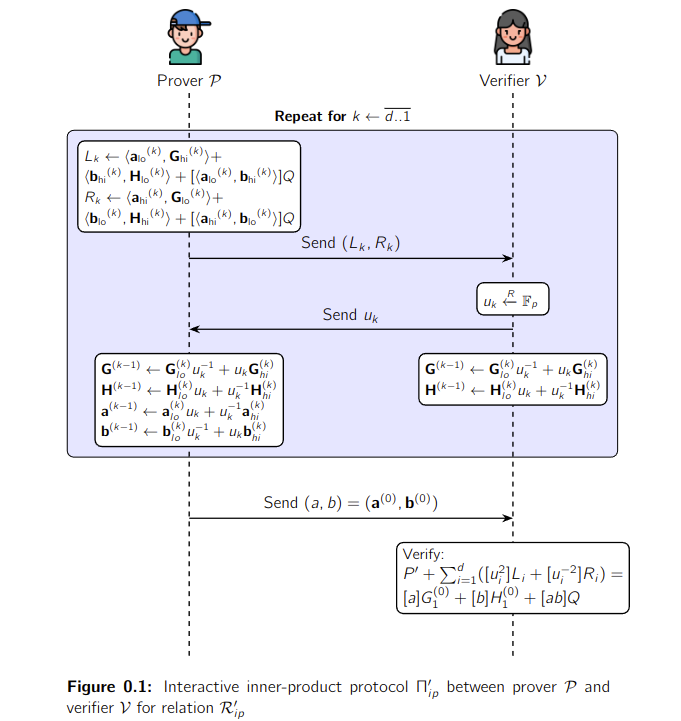
\includegraphics[width=0.8\textwidth]{images/lecture_14/ipa.png}
        \label{fig:ipa}
    \end{figure}
\end{frame}

\begin{frame}{Recap: inner-product argument}
    \begin{itemize}
        \item \textbf{Goal:} Prove $\langle \mathbf{a}, \mathbf{b} \rangle = c$ with logarithmic proof size
        \item Commitment: $P' = \langle \mathbf{a}, \mathbf{G} \rangle + \langle \mathbf{b}, \mathbf{H} \rangle + [\langle \mathbf{a,b} \rangle]Q$
        \item Protocol recursively compresses vectors at each step
        \item Final check: $P' + \sum ([u_i^2]L_i + [u_i^{-2}]R_i) = [a]G + [b]H + [ab]Q$
    \end{itemize}
    \begin{alertblock}{Key properties}
        Proof size is $O(\log_2 n)$, prover and verifier both run in $O(n)$. The protocol doesn't need a \textit{trusted setup}. Protocol is \textit{knowledge sound} and \textit{perfect complete} but not \textit{zero-knowledge}.
    \end{alertblock}
    \begin{block}{Idea}
        We could provide \textit{zero-knowledge} directly to \textit{inner-product argument} construction or use \textbf{zk-mul} protocol for outer construction.
    \end{block}
\end{frame}

\begin{frame}{Recap: zkmul}
    Consider relation $R_{mul} = \{ (\bot; l(x), r(x), t(x)) \vert t(x) = l(x)r(x) \}$ where $l(x) = a + s_L x, r(x) = b + s_R x, t(x) = l(x)r(x)$. Protocol \textbf{zk-mul} is defined as follows:

    \begin{itemize}
        \item Prover computes and sends to $\mathcal{V}$ commitments to $l(x), r(x), t(x)$:
            \begin{align*}
                A &= [a]G + [b]H + [\alpha]B & T_0 &= [ab]G + [\tau_0]B\\
                S &= [s_L]G + [s_R]H + [\beta]B &T_1 &= [s_L + s_R]G + [\tau_1]B\\
                &&T_2 &= [s_Ls_R]G + [\tau_2]B
            \end{align*}
            \item Verifier draws random challenge $u \in \mathbb{F}_p$ and sends it to prover
            \item Prover evaluates and sends to Verifier $(l_u, r_u, t_u, \alpha_u, \tau_u)$: 
            \begin{align*}
                l_u =l(u), r_u = r(u), t_u = l_u \cdot r_u, 
                \alpha_u = \alpha + \beta u, \tau_u = \tau_0 + \tau_1 u + \tau_2 u^2
            \end{align*}
            \item Verifier checks: $A + [u]S \stackrel{?}{=} [l_u]G + [r_u]H + [\alpha_u]B$, $[t_u]G + [\tau_u]B \stackrel{?}{=} T_0 + [u]T_1 + [u^2]T_2$, $t_u \stackrel{?}{=} l_u r_u$
    \end{itemize}
\end{frame}

\begin{frame}{What's next?}
    \begin{figure}[h!]
        \centering
        
\includegraphics[width=0.5\textwidth]{images/lecture_14/ipa_meme.jpg}
    \end{figure}
\end{frame}
\section{IPA polynomial commitment scheme}

\begin{frame}{Recap: Polynomial commitments}
    \begin{itemize}
        \item \textbf{Polynomial commitment scheme} $$\mathcal{C} = (\mathsf{Setup}, \mathsf{Commit}, \mathsf{Open}, \mathsf{VerifyOpen})$$ allows to commit to a polynomial $f(x) = \sum_{i=0}^{n-1} a_i x^i$ and prove its evaluation at some point.
        \item \textbf{Applications:} SNARKs compiled with IOP + polynomial commitment scheme framework (e.g., Halo, Nova, Spartan, Plonk)
        \item \textbf{Desirable properties:} sublinear size, efficient, no trusted setup
    \end{itemize}
    \begin{example}
        One famouos example is the \textbf{KZG} polynomial commitment scheme, which uses bilinear pairings and requires a trusted setup.
    \end{example}
\end{frame}

\begin{frame}{IPA polynomial commitment}
    Let $f(x) = \sum_{i=0}^{n-1} a_i x^i$ be a polynomial of degree $n-1=2^d-1$.
    
    The \textbf{non-hiding IPA polynomial commitment scheme} $\mathcal{C}_{ip} = (\mathsf{Setup, Commit, Open, VerifyOpen})$ is defined as follows:
    \begin{itemize}
        \item $\textcolor{teal}{\mathsf{Setup}}$ returns independent generators $\mathbf{G} = (G_1, \dots, G_n)$.
        \item $\textcolor{teal}{\mathsf{Commit}}$ returns $\mathsf{Com}(f) = \langle \mathbf{f}, \mathbf{G} \rangle$ where $\mathbf{f} = (a_0, \dots, a_{n-1})$
        \item $\textcolor{teal}{\mathsf{Open}}$ given evaluation point $u \in \mathbb{F}_p$ computes $\mathbf{u^n} = (1, u, u^2, \dots, u^{n-1})$,  obtains $f(u) = \langle \mathbf{f, u^n} \rangle$ and runs \textit{inner-product argument} $\Pi_{ip}$ non-interactively setting 
        $$\mathbf{a} = \mathbf{f}, \mathbf{b} = \mathbf{u^n}, P = \mathsf{Com}(f), c = f(u)$$ 
        to produce an evaluation proof $\pi_{ip}$
        \item $\textcolor{teal}{\mathsf{VerifyOpen}}$ given evaluation point $u \in \mathbb{F}_p$ and commitment $\mathsf{Com}(f)$ validates proof $\pi_{ip}$ running the non-interactive verifier $\mathcal{V}$ of \textit{inner-product} argument.
    \end{itemize}
\end{frame}

\section{Range proofs}

\begin{frame}{Range proofs: motivation}
    \begin{itemize}
        \item \textbf{Goal:} Prove $v \in [0, 2^n)$ without revealing $v$:
        $$\mathcal{R}_{rp} = \{ (G, B, V, n; v, \gamma) \vert V = [v]G + [\gamma]B, v \in [0, 2^n) \}$$
        \item \textbf{Applications:} Confidential transactions (e.g., Monero, Mimblewimble), other privacy-preserving protocols.
        \item \textbf{Idea}: Prove $v = \sum_{i=0}^{n-1} v_i 2^i$ and $\forall i \in 0..n-1: v_i \in \{0,1\}$
        \begin{block}{Naive approach}
            One could prove $v = \sum_{i=0}^{n-1} v_i 2^i$ and $\forall i \in 0..n-1: v_i \in \{0,1\}$ using $\Sigma$-protocols, but this would be inefficient due to linear proof.
        \end{block}
    \end{itemize}
\end{frame}

\begin{frame}{Compiling range proof into inner-product}
    Firstly, write $v$ in base-2 representation: $v = \sum_{i=0}^{\lfloor \log_2 v \rfloor} 2^i v_i$ and $\mathbf{a}_L = (v_0, v_1, \dots, v_{n-1})$ be the vector of bits padded with zeroes to length $n$, define $\mathbf{a}_R = \mathbf{a}_L - \mathbf{1}^n$ so the range validation that $v$ lays in $[0, 2^n)$ implies two checks:
    \begin{itemize}
        \item The following inner-product equality holds: $\langle \mathbf{a}_L, \mathbf{2}^n \rangle = v$
        \item Each bit $v_i$ must be either $0$ or $1$:
        \begin{align*}
        \mathbf{a}_L - \mathbf{a}_R - \mathbf{1}^n = \mathbf{0}^n \\
        \mathbf{a}_L \circ \mathbf{a}_R = \mathbf{0}^n
        \end{align*}
        \begin{example}
            Let $\mathbf{a}_L = (1, 0, 1, 0)$, $\mathbf{a}_R = (0, -1, 0, -1)$, then 
            $\mathbf{a}_L \circ \mathbf{a}_R = (0, 0, 0, 0)$
        \end{example}
    \end{itemize}
\end{frame}

\begin{frame}{Compiling range proof into inner-product}
    This two checks imply verification that some vector is zero vector, for that we use some challenge $y \in \mathbb{F}_p$ and check inner-product equalities $$\langle \mathbf{a}_L \circ \mathbf{a}_R, \mathbf{y}^n \rangle = 0 \text{ and } \langle \mathbf{a}_L - \mathbf{a}_R - \mathbf{1}^n, \mathbf{y}^n \rangle = 0$$
    This checks are sound because the prover doesn't know challenge $y$ in advance. So we must combine three inner-product checks:
    \begin{enumerate}
    \item $\langle \mathbf{a}_L, \mathbf{2}^n \rangle = v$
    \item $\langle \mathbf{a}_L, \mathbf{a}_R \circ \mathbf{y}^n \rangle = 0$
    \item $\langle \mathbf{a}_L - \mathbf{a}_R - \mathbf{1}^n, \mathbf{y}^n \rangle = 0$
    \end{enumerate}
    into one soundly summing up with powers of other challenge $z \in \mathbb{F}_p$:
    $$z^2 \cdot \langle \mathbf{a}_L, \mathbf{2}^n \rangle + z \cdot \langle \mathbf{a}_L - \mathbf{a}_R - \mathbf{1}^n, \mathbf{y}^n \rangle + \langle \mathbf{a}_L, \mathbf{a}_R \circ \mathbf{y}^n \rangle = z^2v$$
\end{frame}

\begin{frame}{Compiling range proof into inner-product}
    Using some dark linear algebra wizardry we could combine the three inner-product checks into a single one inner-product check:
    \begin{equation*}
        \langle \mathbf{a}_L - z \cdot \mathbf{1}^n, z^2 \cdot \mathbf{2}^n + z \cdot \mathbf{y}^n + \mathbf{a}_R \circ \mathbf{y}^n\rangle = z^2v + \delta(y,z)
    \end{equation*}
    Where $\delta(y,z)$ could easily be computed by verifier:
    $$\delta(y,z) = (z-z^2)\langle \mathbf{1}^n, \mathbf{y}^n \rangle - z^3 \langle \mathbf{1}^n, \mathbf{2}^n \rangle $$
    Now it's time to bring out \textbf{zk-mul} for inner-products! 
    
    Firstly, construct the blinding polynomials for $\mathbf{a}_L$ and $\mathbf{a}_R$:
    $$\mathbf{a}_L' \gets \mathbf{a}_L + \mathbf{s}_L x \quad \mathbf{a}_R' \gets \mathbf{a}_R + \mathbf{s}_R x$$
    Compute polynomials $\mathbf{l}(x) = \mathbf{l}_0 + \mathbf{l}_1 x, \quad \mathbf{r}(x) = \mathbf{r}_0 + \mathbf{r}_1 x$:
    \begin{align*}
        \mathbf{l}(x) &= \mathbf{a}_L' - z \cdot \mathbf{1}^n = (\mathbf{a}_L + \mathbf{s}_L x) - z \cdot \mathbf{1}^n = \textcolor{teal}{\mathbf{a}_L - z \cdot \mathbf{1}^n} + \mathbf{s}_L x\\
        \mathbf{r}(x) &= z^2 \cdot \mathbf{2}^n + z \cdot \mathbf{y}^n + \mathbf{a}_R' \circ \mathbf{y}^n = z^2 \cdot \mathbf{2}^n + z \cdot \mathbf{y}^n + (\mathbf{a}_R + \mathbf{s}_R x) \circ \mathbf{y}^n \\
        & = \textcolor{orange}{z^2 \cdot \mathbf{2}^n + z \cdot \mathbf{y}^n + \mathbf{a}_R \circ \mathbf{y}^n} + \mathbf{s}_R \circ \mathbf{y}^n x
    \end{align*}
\end{frame}

\begin{frame}{Compiling range proof into inner-product}
    $$t(x) = \langle \mathbf{l}(x), \mathbf{r}(x) \rangle = t_0 + t_1 x + t_2 x^2$$
    Now $\mathcal{P}$ needs to apply \textbf{zk-mul} for proving: $$t_0 =  \langle \textcolor{teal}{\mathbf{a}_L - z \cdot \mathbf{1}^n}, \textcolor{orange}{z^2 \cdot \mathbf{2}^n + z \cdot \mathbf{y}^n + \mathbf{a}_R \circ \mathbf{y}^n}\rangle = z^2v + \delta(y,z)$$ 
    \textbf{Note}: $\mathcal{V}$ could compute commitment $Com(t_0)$ using $V=Com(v)$
    \begin{alertblock}{Remark}
    We couldn't apply raw \textbf{zk-mul} as $\mathbf{l}_0$ depends on verifier-provided challenges, instead $\mathcal{P}$ firstly commits to $\mathbf{a}_L, \mathbf{a}_R$ and blinders $\mathbf{s}_L, \mathbf{s}_R$, obtaints challenges $y,z$ from $\mathcal{V}$ and computes rest of the commitments. 
    
    During verification phase $\mathcal{V}$ should adjust commitments to $\mathbf{l}(x), \mathbf{r}(x)$ by himself using homomorphic proterties of Pedersen commitment scheme.
    \end{alertblock}
\end{frame}

\begin{frame}{Range proofs: building the protocol}
    \begin{itemize}
        \item $\mathsf{Setup}$ returns independent generators $\mathbf{G}, \mathbf{H} \in \mathbb{G}^n$
        \item Prover does bit decomposition of $v$: $\mathbf{a}_L \gets \mathbf{v}, \mathbf{a}_R \gets \mathbf{a}_L - \mathbf{1}^n$, choses blinding terms $\mathbf{s}_L, \mathbf{s}_R \in \mathbb{F}_p^n, \alpha, \beta \in \mathbb{F}_p$, sends commitments:
            \begin{align*}
                A = \langle \mathbf{a}_L, \mathbf{G} \rangle + \langle \mathbf{a}_R, \mathbf{H} \rangle + [\alpha]B &&
                S = \langle \mathbf{s}_L, \mathbf{G} \rangle + \langle \mathbf{s}_R, \mathbf{H} \rangle + [\beta]B
            \end{align*}
        \item Verifier $\mathcal{V}$ samples challenges $y, z \xleftarrow{R} \mathbb{F}_p$ and sends them to $\mathcal{P}$
        \item Prover $\mathcal{P}$ reconstructs polynomials $\mathbf{l}(x), \mathbf{r}(x), \mathbf{t}(x)$:
            \begin{equation*}
                \begin{aligned}
                    \mathbf{l}(x) &= \mathbf{a}_L - z \cdot \mathbf{1}^n + \mathbf{s}_L x\\
                    \mathbf{r}(x) &= z^2 \cdot \mathbf{2}^n + z \cdot \mathbf{y}^n + \mathbf{a}_R \circ \mathbf{y}^n + \mathbf{s}_R \circ \mathbf{y}^n x\\
                    t(x) &= \langle \mathbf{l}(x), \mathbf{r}(x) \rangle = t_0 + t_1 x + t_2 x^2
                \end{aligned}
            \end{equation*}
            \begin{equation*}
                \begin{aligned}
                    t_0 &=  \langle \textcolor{teal}{\mathbf{a}_L - z \cdot \mathbf{1}^n}, \textcolor{orange}{z^2 \cdot \mathbf{2}^n + z \cdot \mathbf{y}^n + \mathbf{a}_R \circ \mathbf{y}^n}\rangle = z^2v + \delta(y,z)\\
                    t_1 &= \langle \mathbf{a}_L - z \cdot \mathbf{1}^n, \mathbf{y}^n \circ \mathbf{s}_R \rangle + \langle \mathbf{y}^n \circ (\mathbf{a}_R + z\cdot \mathbf{1}^n ) + z^2 \cdot \mathbf{2}^n, \mathbf{s}_L\rangle \\
                    t_2 & = \langle \mathbf{s}_L, \mathbf{y}^n \circ \mathbf{s}_R \rangle
                \end{aligned}
            \end{equation*}
    \end{itemize}
\end{frame}

\begin{frame}{Range proofs: proving}
    \begin{itemize}
        \item Prover $\mathcal{P}$ draws blinding factors $\tau_1, \tau_2 \xleftarrow{R} \mathbb{F}_p$ and sends to $\mathcal{V}$ commitments for coefficients of $t(x)$:
            \begin{equation*}
                \begin{aligned}
                    T_1 &= [t_1]G + [\tau_1]B \\
                    T_2 &= [t_2]G + [\tau_2]B
                \end{aligned}
            \end{equation*}
            \textbf{Note:} prover does not have to send commitment to $t_0$ as it's the inner-product we want to prove and it could be computed from high-level commitment $V$.
        \item Verifier $\mathcal{V}$ samples and sends to $\mathcal{P}$ evaluation point $u \xleftarrow{R} \mathbb{F}_p$
        \item Prover $\mathcal{P}$ evaluates polynomials at $u$:
        \begin{equation*}
            \begin{aligned}
                \mathbf{l}_u & = \mathbf{l}(u) & \alpha_u &= \alpha + \beta u\\
                \mathbf{r}_u &= \mathbf{r}(u) & \tau_u &= z^2\gamma + \tau_1 u + \tau_2 u^2\\
                t_u &= t(u) = t_0 + t_1u + t_2u^2 & 
            \end{aligned}
        \end{equation*}
        and sends $(\mathbf{l}_u, \mathbf{r}_u, t_u, \alpha_u, \tau_u)$ to $\mathcal{V}$.
    \end{itemize}
\end{frame}

\begin{frame}{Range proofs: verification}
    \begin{itemize}
        \item Verifier $\mathcal{V}$ checks:
            \begin{equation*}
                \begin{aligned}
                    A + [u]S + \langle -z \cdot \mathbf{1}^n, \mathbf{G} \rangle &+ \langle z \cdot \mathbf{y}^n + z^2 \cdot \mathbf{2}^n, \mathbf{y}^{-n} \circ \mathbf{H} \rangle \\
                    &\stackrel{\text{?}}{=} \langle \mathbf{l}_u, \mathbf{G} \rangle + \langle \mathbf{r}_u, \mathbf{y}^{-n} \circ \mathbf{H} \rangle + [\alpha_u]B \\
                    [t_u]G + [\tau_u]B &\stackrel{\text{?}}{=} [z^2]V + [\delta(y,z)]G + [u]T_1 + [u^2]T_2 \\
                    t_u &\stackrel{\text{?}}{=} \langle \mathbf{l}_u \mathbf{r}_u \rangle
                \end{aligned}
            \end{equation*}
    \end{itemize}
    \begin{block}{Remark}
        To provide logarithmic size-proof instead of sending $\mathbf{l}_u, \mathbf{r}_u$ parties could run an inner-product argument \textbf{IPA} on inputs $(\mathbf{G},\mathbf{y}^{-n} \circ \mathbf{H}, P, t_u; \mathbf{l}_u, \mathbf{r}_u)$ where:
        $$P = A + [u]S + \langle -z \cdot \mathbf{1}^n, \mathbf{G} \rangle + \langle z \cdot \mathbf{y}^n + z^2 \cdot \mathbf{2}^n, \mathbf{y}^{-n} \circ \mathbf{H} \rangle - [\alpha_u]B$$
    \end{block}
\end{frame}

\begin{frame}{Range proofs: efficiency \& extensions}
    \begin{theorem}
        The \textbf{range proof protocol} $\Pi_{rp}$ has \textit{perfect completeness, computational extended witness emulation, perfect honest-verifier zero-knowledge}
        \label{th:range_proof}
    \end{theorem}
    Note that protocol is efficient as it has logarithmic proof size. 
    \begin{block}{Remark}
        The \textbf{range proof protocol} could be extended to support proving multiple range proofs at once with some efficiency improvements.
    \end{block}
\end{frame}
\begin{frame}{Range proofs \& subset-sum NP-complete problem}
    One of the most famous \textit{NP-complete} problems is the \textbf{subset-sum problem}: given a set of numbers presented as vector $\mathbf{s}$ and number $v \in \mathbb{N}$, does a some subset sums up to $v$. It turns out that we could use our \textbf{range-proof} protocol for this problem. One could simply replace first inner-product check $\langle \mathbf{a}_L, \mathbf{2}^n \rangle = v$ with $\langle \mathbf{a}_L, \mathbf{s} \rangle = v$ where $\mathbf{a}_L$ is the secret vector of bits that encode positions of $\mathbf{s}$ that sum up to $v$.
    \begin{example}
        Let $\mathbf{s} = (6,8,2,3)$ and $v = 14$. Then setting $\mathbf{a}_L = (1,1,0,0)$ we could use $\Pi_{rp}$ to prove that there exists a subset of $\mathbf{s}$ that sums up to $v=14$ without disclosing that subset.
    \end{example}
    Therefore, \textbf{bulletproofs range proof} protocol is capable to prove a knowledge of witness to any $NP$-problem as they all could be reduced to the $\textbf{subset-sum problem}$
\end{frame}
\section{Arithmetic circuits}

\begin{frame}{Bulletproofs for arithmetic circuits}
    \begin{itemize}
        \item \textbf{Goal:} Prove that a circuit computes correctly without revealing inputs or intermediate values (\textit{circuit satisfiability problem}).
        \item \textbf{Approach:} Use inner-product argument to prove correctness of arithmetic circuits
        \item \textbf{Applications:} Privacy-preserving smart contracts, confidential computations, zero-knowledge proofs for complex computations
    \end{itemize}
    \textbf{Bulletproofs} arithmetization slightly differs from the classic R1CS, however it could be transformed vice-versa easily. Also \textbf{bulletproofs} arithmetization is more convenient and human-friendly for encoding most of the arithmetic circuits than the R1CS.
\end{frame}

\begin{frame}{Arithmetic circuits: variables}
    There is two types of variables in \textit{bulletproofs} constraint system:
    \begin{itemize}
        \item \textbf{High-level variables} $\mathbf{v} \in \mathbb{F}_p^m$ are the private witness inputs to the circuit, typically provided with Pedersen commitments $\mathbf{V} \in \mathbb{G}^m$.
        \item \textbf{Low-level variables} $\mathbf{a}_L, \mathbf{a}_R, \mathbf{a}_O \in \mathbb{F}_p^n$ are the intermediate witness values of computation.
    \end{itemize}
    We will define circuit as a set of multiplication constraints operating with \textit{low-level} variables and set of linear constraints which links \textit{low-level} variables between each other and \textit{high-level} variables as well.
\end{frame}

\begin{frame}{Arithmetic circuits: constraints}
    Multiplication constraints are defined with one vector equation:
    $$ \mathbf{a}_L \circ \mathbf{a}_R = \mathbf{a}_O $$
    Linear constraints are defined via:
    $$ \mathbf{W}_L \cdot \mathbf{a}_L + \mathbf{W}_R \cdot \mathbf{a}_R + \mathbf{W}_O \cdot \mathbf{a}_O = \mathbf{W}_V \cdot \mathbf{v} + \mathbf{c} $$
    Where $\mathbf{a_L, a_R, a_O}$ -- vectors of left and right inputs for multiplication gates and output values (all of them are low-level variables). $\mathbf{W_L, W_R, W_O} \in \mathbb{F}_p^{q \times n}, \mathbf{W}_V \in \mathbb{F}_p^{q \times m}$ -- public matrices of weights for linear constraints(obviously known to verifier). $\mathbf{c} \in \mathbb{F}_p^q$ -- public vector of constants. Typically they encode wiring of the circuit and other linear relations between variables.
\end{frame}

\begin{frame}{Arithmetic circuits: example}
    \begin{example}
        Consider the following elliptic curve membership circuit. Here witness $(v_1, v_2)$ should satisfy elliptic curve equation:
        \begin{equation*}
            y^2 = x^3 + ax + b
        \end{equation*}

        The arithmetization for this circuit is as follows:

        \textbf{Low-level variables:}
        \begin{equation*}
            \mathbf{a}_L = \begin{bmatrix} x \\ x \\ y \end{bmatrix}, \quad 
            \mathbf{a}_R = \begin{bmatrix} x \\ x^2 \\ y \end{bmatrix}, \quad 
            \mathbf{a}_O = \begin{bmatrix} x^2\\x^3 \\ y^2 \end{bmatrix}
        \end{equation*}

        \textbf{High-level variables:}
        \begin{equation*}
            \mathbf{v} = \begin{bmatrix} v_1 \\ v_2 \end{bmatrix}
        \end{equation*}
    \end{example}
\end{frame}

\begin{frame}{Arithmetic circuits: example}
    \begin{example}        
        \textbf{Multiplication constraints:}
        \begin{equation*}
            \mathbf{a}_L \circ \mathbf{a}_R = \mathbf{a}_O \Rightarrow \begin{bmatrix} 
                x \cdot x = x^2 \\
                x \cdot x^2 = x^3 \\ 
                y \cdot y = y^2
            \end{bmatrix}
        \end{equation*}
            \textbf{Linear constraints:}

    \begin{equation*}
        \begin{aligned}
            \mathbf{a}_L^{(1)} &= v_1 & \mathbf{a}_R^{(1)} &= v_1 \\
            \mathbf{a}_L^{(2)} - \mathbf{a}_L^{(1)} &= 0 & \mathbf{a}_R^{(2)} - \mathbf{a}_O^{(1)} &= 0 \\
            \mathbf{a}_L^{(3)} &= v_2 & \mathbf{a}_R^{(3)} &= v_2 \\
            \mathbf{a}_O^{(3)} - \mathbf{a}_O^{(2)} - a \cdot \mathbf{a}_L^{(1)} &= b &
        \end{aligned}
    \end{equation*}
    
    \begin{equation*}
    \mathbf{W}_L \cdot \mathbf{a}_L + \mathbf{W}_R \cdot \mathbf{a}_R + \mathbf{W}_O \cdot \mathbf{a}_O = \mathbf{W}_V \cdot \mathbf{v} + \mathbf{c}
    \end{equation*}
    \end{example}
\end{frame}

\begin{frame}{Arithmetic circuits: example}
    \begin{example}
    \begin{align*}
    \mathbf{W}_L = \begin{bmatrix}
        1 & 0 & 0 \\
        0 & 0 & 0 \\
        -1 & 1 & 0 \\
        0 & 0 & 0 \\
        0 & 0 & 1 \\
        0 & 0 & 0 \\
        -a & 0 & 0
    \end{bmatrix},\quad
    \mathbf{W}_R = \begin{bmatrix}
        0 & 0 & 0 \\
        1 & 0 & 0 \\
        0 & 0 & 0 \\
        0 & 1 & 0 \\
        0 & 0 & 0 \\
        0 & 0 & 1 \\
        0 & 0 & 0
    \end{bmatrix},\quad
    \mathbf{W}_O = \begin{bmatrix}
        0 & 0 & 0 \\
        0 & 0 & 0 \\
        0 & 0 & 0 \\
        -1 & 0 & 0 \\
        0 & 0 & 0 \\
        0 & 0 & 0 \\
        0 & -1 & 1
    \end{bmatrix},\\
    \mathbf{W}_V = \begin{bmatrix}
        1 & 0 \\
        1 & 0 \\
        0 & 0 \\
        0 & 0 \\
        0 & 1 \\
        0 & 1 \\
        0 & 0
    \end{bmatrix},\quad
    \mathbf{c} = \begin{bmatrix}
        0 \\ 0 \\ 0 \\ 0 \\ 0 \\ 0 \\ b
    \end{bmatrix}
    \end{align*}
    \end{example}
\end{frame}

\begin{frame}{Bulletproofs for circuits: relation}
    Consider the relation:
    \begin{equation*}
        \begin{aligned}
            \mathcal{R}_{sat} = \left\{
                \begin{array}{l} 
                    (G, B, \mathbf{V}, \mathbf{W}_L, \mathbf{W}_R, \mathbf{W}_O, \mathbf{W}_V, \mathbf{c}; \mathbf{a}_L, \mathbf{a}_R, \mathbf{a}_O, \mathbf{v}, \mathbf{r}) | \\ 
                    \forall i=1..m: V_i = [v_i]G + [r_i]B \wedge \\
                    \mathbf{a}_L \circ \mathbf{a}_R = \mathbf{a}_O \wedge \\
                    \mathbf{W}_L \cdot \mathbf{a}_L + \mathbf{W}_R \cdot \mathbf{a}_R + \mathbf{W}_O \cdot \mathbf{a}_O = \mathbf{W}_V \cdot \mathbf{v} + \mathbf{c}
            \end{array}\right\}
        \end{aligned}
    \end{equation*}
    Where $\mathbf{a}_L, \mathbf{a}_R, \mathbf{a}_O \in \mathbb{F}_p^n$, $\mathbf{v}, \mathbf{r} \in \mathbb{F}_p^m$, $\mathbf{W}_L, \mathbf{W}_R, \mathbf{W}_O \in \mathbb{F}_p^{q \times n}$, $\mathbf{W}_V \in \mathbb{F}_p^{q \times m}$, $\mathbf{c} \in \mathbb{F}_p^q$.
    \begin{block}{Note}
        Informally this relation states that there exists a valid witness $\mathbf{v}$ that satisfies all constraints of the circuit. For the verifier witness is presented only as commitments vector $\mathbf{V}$.
    \end{block}
\end{frame}

\begin{frame}{Arithmetic circuits: compiling into inner-product}
We could use similar to \textit{range-proofs} technique to compile constraints of the circuit into inner-product relation. For multiplicative constraints take random $y \in \mathbb{F}_p$ and apply zero check:
$$ \langle \mathbf{a}_L \circ \mathbf{a}_R - \mathbf{a}_O, \mathbf{y}^n \rangle = 0$$
Same for linear constraints, but for different randomness $z \in \mathbb{F}_p$:
$$ \langle \mathbf{W}_L \cdot \mathbf{a}_L + \mathbf{W}_R \cdot \mathbf{a}_R + \mathbf{W}_O \cdot \mathbf{a}_O - \mathbf{W}_V \cdot \mathbf{v} - \mathbf{c}, \mathbf{z}^q \rangle = 0$$
Combine this two checks to one using the same randomness $z$:
\begin{equation*}
    \begin{aligned}
        \langle \mathbf{a}_L \circ \mathbf{a}_R - \mathbf{a}_O, \mathbf{y}^n \rangle + \langle z \cdot \mathbf{z}^q,  \mathbf{W}_L \cdot \mathbf{a}_L + \mathbf{W}_R \cdot \mathbf{a}_R + \mathbf{W}_O \cdot \mathbf{a}_O - \mathbf{W}_V \cdot \mathbf{v} - \mathbf{c} \rangle \\= 0
    \end{aligned}
\end{equation*}
This check is sound as typically a prover could not control values of $y,z$ before he commits to $\mathbf{a_L, a_R, a_O}$ and $\mathbf{v}$.
\end{frame}

\begin{frame}{Arithmetic circuits: compiling into inner-product}
    Denote $w_c = \langle z \cdot \mathbf{z}^q, \mathbf{c} \rangle$ and flattened linear constraints(still public and easily computed by verifier):
    \begin{equation*}
        \begin{aligned}
            \mathbf{w}_L &= \mathbf{W}_L^T \cdot (z \cdot \mathbf{z}^q) &
            \mathbf{w}_R &= \mathbf{W}_R^T \cdot (z \cdot \mathbf{z}^q) \\
            \mathbf{w}_O &= \mathbf{W}_O^T \cdot (z \cdot \mathbf{z}^q) &
            \mathbf{w}_V &= \mathbf{W}_V^T \cdot (z \cdot \mathbf{z}^q) 
        \end{aligned}
    \end{equation*}
    Again doing some linear algebra witchcraft we could separate $\mathbf{a}_L, \mathbf{a}_O$ to be on the left side of the inner-product and $\mathbf{a}_R$ to be on the right:
        \begin{equation*}
            \begin{aligned}
                w_c + \langle \mathbf{w}_V, \mathbf{v} \rangle + \delta(y, z) =\\
                \langle \textcolor{teal}{\mathbf{a}_L + \mathbf{y}^{-n} \circ \mathbf{w}_R}, \textcolor{orange}{\mathbf{y}^n \circ \mathbf{a}_R + \mathbf{w}_L} \rangle + \langle \textcolor{purple}{\mathbf{a}_O}, \textcolor{blue}{ -\mathbf{y}^n + \mathbf{w}_O} \rangle
            \end{aligned}
        \end{equation*}
        Where $\delta(y, z) = \langle \mathbf{y}^{-n} \circ \mathbf{w}_R, \mathbf{w}_L \rangle$ -- easily computable by $\mathcal{V}$.

        Here we have a sum of 2 separate inner-products, we could express it as second-degree coefficient of the following polynomial:
        \begin{equation*}
            \begin{aligned}
            \langle \textcolor{teal}{\mathbf{a}}x + \textcolor{purple}{\mathbf{c}}x^2, \textcolor{blue}{\mathbf{d}} + \textcolor{orange}{\mathbf{b}}x \rangle = s_1x + s_2x^2 + s_3x^3 =\\
            x \cdot \langle \textcolor{teal}{\mathbf{a}}, \textcolor{blue}{\mathbf{d}} \rangle + x^2 \cdot (\langle \textcolor{teal}{\mathbf{a}}, \textcolor{orange}{\mathbf{b}} \rangle + \langle \textcolor{purple}{\mathbf{c}}, \textcolor{blue}{\mathbf{d}} \rangle) + x^3 \cdot \langle \textcolor{purple}{\mathbf{c}}, \textcolor{orange}{\mathbf{b}} \rangle
            \end{aligned}
        \end{equation*}
\end{frame}

\begin{frame}{Arithmetic circuits: compiling into inner-product}
    \vspace{-1em}
    \begin{equation*}
        \begin{aligned}
            &\textcolor{teal}{\mathbf{a}} \gets \textcolor{teal}{\mathbf{a}_L + \mathbf{y}^{-n} \circ \mathbf{w}_R} &&\textcolor{orange}{\mathbf{b}} \gets \textcolor{orange}{\mathbf{y}^n \circ \mathbf{a}_R + \mathbf{w}_L} \\
            &\textcolor{purple}{\mathbf{c}} \gets \textcolor{purple}{\mathbf{a}_O} &&\textcolor{blue}{\mathbf{d}} \gets \textcolor{blue}{-\mathbf{y}^n + \mathbf{w}_O}
        \end{aligned}
    \end{equation*}
    Desired sum of inner products is the second-degree coefficient $s_2$:
    $$ w_c + \langle \mathbf{w}_V, \mathbf{v} \rangle + \delta(y, z) = s_2$$
    To obtain final polynomials $\mathbf{l}(x), \mathbf{r}(x)$ we must firstly blind $\mathbf{a}_L, \mathbf{a}_R$:
    \begin{equation*}
        \begin{aligned}
        \mathbf{a}_L \gets \mathbf{a}_L + \mathbf{s}_Lx^2 && \mathbf{a}_R \gets \mathbf{a}_R + \mathbf{s}_Rx^2
        \end{aligned}
    \end{equation*}
    And finally compute polynomials $\mathbf{l}(x), \mathbf{r}(x)$ as follows:
    \begin{equation*}
        \begin{aligned}
            {\mathbf{l}}(x) &= \mathbf{s}_L \cdot x^3 + \mathbf{a}_O \cdot x^2 + (\mathbf{a}_L + \mathbf{y}^{-n} \circ \mathbf{w}_R) \cdot x \\
            {\mathbf{r}}(x) &= \mathbf{y}^n \circ \mathbf{s}_R \cdot x^3 + (\mathbf{y}^n \circ \mathbf{a}_R +  \mathbf{w}_L) \cdot x - \mathbf{y}^n + \mathbf{w}_O \\
            t(x) &= \langle \mathbf{l}(x), \mathbf{r}(x) \rangle = \sum_{i=0}^6 t_i x_i
        \end{aligned}
    \end{equation*}
    Where $t_2 = w_c + \langle \mathbf{w}_V, \mathbf{v} \rangle + \delta(y, z)$ -- desired sum of inner-products.
\end{frame}

\begin{frame}{Arithmetic circuits: witness commitments}
    Here we could again apply modified \textbf{zk-mul} to prove that $t_2$ is a valid sum of inner-products:
    \begin{itemize}
        \item $\mathsf{Setup}$: returns vectors of independent generators $\mathbf{G,H} \in \mathbb{G}^n$.
        \item Prover $\mathcal{P}$ choses blinding factors $\alpha, \beta, \gamma \in \mathbb{F}_p, \mathbf{s}_L, \mathbf{s}_R \in \mathbb{F}_p^n$ and sends the following commitments to $\mathcal{V}$:
        \begin{equation*}
            \begin{aligned}
                A_I &= \langle \mathbf{a}_L, \mathbf{G} \rangle + \langle \mathbf{a}_R, \mathbf{H} \rangle + [\alpha]B\\
                A_O &= \langle \mathbf{a}_O, \mathbf{G} \rangle + [\gamma]B\\
                S &= \langle \mathbf{s}_L, \mathbf{G} \rangle + \langle \mathbf{s}_R, \mathbf{H} \rangle + [\beta]B
            \end{aligned}
        \end{equation*}
        \item Verifier samples challenges $y,z \xleftarrow{R} \mathbb{F}_p$ and sends them to $\mathcal{P}$.
    \end{itemize}
\end{frame}

\begin{frame}{Arithmetic circuits: product commitments}
    \begin{itemize}
        \item Using challenges $y,z$ prover forms polynomials $\mathbf{l}(x), \mathbf{r}(x), t(x)$:
        \begin{equation*}
            \begin{aligned}
                \mathbf{l}(x) &= \mathbf{s}_L \cdot x^3 + \mathbf{a}_O \cdot x^2 + (\mathbf{a}_L + \mathbf{y}^{-n} \circ \mathbf{w}_R) \cdot x \\
                \mathbf{r}(x) &= \mathbf{y}^n \circ \mathbf{s}_R \cdot x^3 + (\mathbf{y}^n \circ \mathbf{a}_R +  \mathbf{w}_L) \cdot x - \mathbf{y}^n + \mathbf{w}_O \\
                t(x) &= \langle \mathbf{l}(x), \mathbf{r}(x) \rangle = t_1 x + t_2 x^2 + t_3 x^3 + t_4 x^4 + t_5 x^5 + t_6 x^6
            \end{aligned}
        \end{equation*}
        $\mathcal{P}$ choses random blinding factors $\tau_1, \tau_3, \tau_4, \tau_5, \tau_6 \in \mathbb{F}_p$ and sends to $\mathcal{V}$ commitments to its coefficients:
        \begin{equation*}
            \begin{aligned}
                T_1 &= [t_1]G + [\tau_1]B &
                T_3 &= [t_3]G + [\tau_3]B &
                T_4 &= [t_4]G + [\tau_4]B\\
                T_5 &= [t_5]G + [\tau_5]B &
                T_6 &= [t_6]G + [\tau_6]B &
            \end{aligned}
        \end{equation*}
        \textbf{Note:} Prover does not send separate commitment to $t_2$ as the verifier could derive it from $\mathbf{V}$ and the circuit public parameters: 
        \begin{align*}
            t_2 &= w_c + \langle \mathbf{w}_V, \mathbf{v} \rangle + \delta(y, z) \\
            T_2 &= \langle \mathbf{w}_V, \mathbf{V} \rangle + [\delta(y, z) + w_c]G
        \end{align*}
    \end{itemize}
\end{frame}

\begin{frame}{Arithmetic circuits: evaluating polynomials}
    \begin{itemize}
        \item Verifier samples and sends to $\mathcal{P}$ random evaluation point $u \xleftarrow{R} \mathbb{F}_p$.
        \item Prover evaluates polynomials at $u$:
            \begin{equation*}
                \begin{aligned}
                    \mathbf{l}_u &= \mathbf{l}(u) \\
                    \mathbf{r}_u &= \mathbf{r}(u) \\
                    t_u &= \langle \mathbf{l}_u, \mathbf{r}_u \rangle = t(u) \\
                    \tau_u &= \tau_1 \cdot u + \langle \mathbf{w}_V, \mathbf{r} \rangle u^2 + \tau_3 \cdot u^3 + \tau_4 \cdot u^4 + \tau_5 \cdot u^5 + \tau_6 \cdot u^6\\
                    \alpha_u &= \alpha u + \gamma u^2 + \beta u^3
                \end{aligned}
            \end{equation*}
            and sends $(\mathbf{l}_u, \mathbf{r}_u, t_u, \alpha_u, \tau_u)$ to $\mathcal{V}$.
    \end{itemize}
\end{frame}

\begin{frame}{Arithmetic circuits: verification}
    \begin{itemize}
        \item Verifier performs checks:
            \begin{equation*}
                \begin{aligned}
                    &[u]A_I + [u^2]A_O + [u^3]S - \langle \mathbf{1}, \mathbf{H} \rangle + \\
                    &u \cdot (\langle \mathbf{y}^{-n} \circ \mathbf{w}_L, \mathbf{G} \rangle + \langle \mathbf{y}^{-n} \circ \mathbf{w}_R, \mathbf{H} \rangle) + \langle \mathbf{y}^{-n} \circ \mathbf{w}_O, \mathbf{H} \rangle \\
                    &\stackrel{\text{?}}{=} \langle \mathbf{l}_u, \mathbf{G} \rangle + \langle \mathbf{r}_u, \mathbf{y}^{-n} \circ \mathbf{H} \rangle + [\alpha_u]B\\
                    [t_u]G + [\tau_u]B &\stackrel{\text{?}}{=} [u]T_1 + u^2 \cdot (\langle \mathbf{w}_V, \mathbf{V} \rangle + [\delta(y,z) + w_c]G) +\\
                    &[u^3]T_3 + [u^4]T_4 + [u^5]T_5 + [u^6]T_6\\
                    t_u &\stackrel{\text{?}}{=} \langle \mathbf{l}_u, \mathbf{r}_u \rangle
                \end{aligned}
            \end{equation*}
    \end{itemize}
    \begin{block}{Remark}
        To provide logarithmic proof instead of sending $\mathbf{l}_u, \mathbf{r}_u$ parties could run \textbf{IPA} on inputs $(\mathbf{G},\mathbf{y}^{-n} \circ \mathbf{H}, P, t_u; \mathbf{l}_u, \mathbf{r}_u)$ where:
        \begin{align*}
            P =& [u]A_I + [u^2]A_O + [u^3]S - \langle \mathbf{1}, \mathbf{H} \rangle +\\
                &u \cdot (\langle \mathbf{y}^{-n} \circ \mathbf{w}_L, \mathbf{G} \rangle + \langle \mathbf{y}^{-n} \circ \mathbf{w}_R, \mathbf{H} \rangle) + \langle \mathbf{y}^{-n} \circ \mathbf{w}_O, \mathbf{H} \rangle - [\alpha_u]B
        \end{align*}
    \end{block}
\end{frame}

\begin{frame}{Arithmetic circuits: efficiency \& extensions}
    \begin{theorem}
        The \textbf{arithmetic circuits protocol} has \textit{perfect completeness, computational extended witness emulation, perfect honest-verifier zero-knowledge}
    \end{theorem}
    The protocol is efficient as it has logarithmic proof size. 
    \begin{block}{Remark}
        The \textbf{arithmetic circuits protocol} protocol could be slightly modified to provide intermediate random challenges inside the circuit. For example it would allow proving \textit{permutation check}: $\{a,b\} = \{c,d\}  \iff (a-x)\cdot(b-x) = (c-x)\cdot(d-x)$ for some random challenge $x$.
    \end{block}
\end{frame}

\begin{frame}{Questions?}
    \begin{figure}
        \centering
        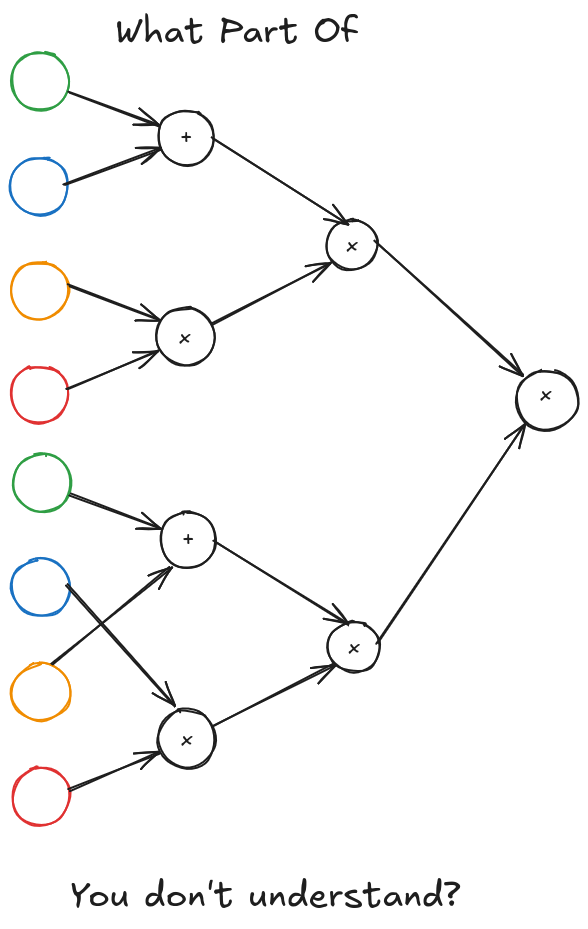
\includegraphics[width=0.44\textwidth]{images/lecture_14/circuit.png}
        \label{fig:np-completeness}
    \end{figure}
\end{frame}
\end{document}